\documentclass[a4paper, 11pt]{article}
% English font
% \usepackage[T1]{fontenc}
% \usepackage{mathptmx}

% Geometry
\usepackage{fullpage}
%\usepackage[top=3cm,bottom=2.5cm,left=2.6cm,right=2.6cm]{geometry}
\usepackage{setspace}

\onehalfspacing

% Mathttt
\usepackage{amsmath, amssymb, amsthm, bm, bbm}
\usepackage{mathtools}
\theoremstyle{plain} % Theorem ilatics
% \theoremstyle{definition}

\newtheorem{assumption}{Assumption}
\newtheorem{definition}{Definition}
\newtheorem{theorem}{Theorem}
\newtheorem{prop}{Proposition}
\newtheorem{guess}{Conjecture}
\newtheorem{lemma}{Lemma}
\newtheorem{cor}{Corollary}
\newtheorem{aux}{Auxiliary Result}
\newtheorem{remark}{Remark}

\DeclareMathOperator*{\argmax}{arg\,max}
\DeclareMathOperator*{\argmin}{arg\,min}

% Linkage
\usepackage{hyperref}
\hypersetup{colorlinks=true,citecolor=blue,urlcolor=blue}

% Footnote
\usepackage[bottom]{footmisc}

% References
\usepackage{natbib}
\bibliographystyle{apalike}
\renewcommand{\bibname}{References}

% Itemize
\usepackage{enumitem}

% Diagram Figure
\usepackage{tikz}
\usepackage{varwidth}

% Others
\usepackage{fancyhdr}
\usepackage{graphicx, graphics, caption, subcaption}
\usepackage{appendix}
\usepackage{tabularx}
\usepackage[section]{placeins}
\usepackage{color,pstricks}
\usepackage{setspace}

\usepackage{float}
\usepackage{booktabs}
\usepackage{multirow}
\usepackage{numprint}


\title{Information Disclosure in Dynamic Innovation Contests}
\author{Jussi Keppo \and Zhuang Linsheng}
\date{}

\begin{document}

\maketitle

\begin{abstract}
...
\end{abstract}

\section{Introduction}

\begin{itemize}
\item Kaggle\footnote{\url{https://www.kaggle.com}} ...
\item Meta-kaggle \cite{megan_risdal_timo_bozsolik_2022}. 
\end{itemize}

\subsection{Literature Review}

This paper focuses on the two players innovation contest with a continuous time  where the players’ relative position is public information throughout the game.
This is closely related to tug-or-war contest, which, to our knowledge, was first formally given by \citet{Harris1987Race} as a one-dimensional simplification of the multi-stage R\&D race. 
The output processes are model by Brownian motions drifted with effort inputs, which is followed by \cite{budd1993model} who model the state of a dynamic competition of two innovative duopoly firms by a Brownian motion drifted by the effort gap, and solve the equilibrium approximately. 
Furthermore, \citet{Moscarini2007Contest} model the tug-of-war state as the gap of the two outputs directly, and draw an analytical equilibrium of the pure strategies. 

...

Information disclosure in contest - \cite{Bimpikis2019Contest}. 

...

Closest paper - \cite{ryvkin2022fight}.

...




\section{The Model}

% Effort, Output and Gap
We assume two players, $i$ and $j$, compete for a prize $\theta>0$. 
Winner gets the prize and loser gets nothing. 
The contest starts at time zero. 
At every time $t\ge0$, the representative player $i$ chooses an effort level $q_{i,t}$ and burdens a quadratic cost $C_i(q_{i,t}) = c_i q_{i,t}^2/2$, with a lower $c_i$ corresponding to higher ability. 
The output of player $i$ denoted by $x_{i,t}$ follows 
\begin{equation}\label{output-process}
dx_{i,t} = q_{i,t} dt + \sigma_idW_{i,t} 
\end{equation}
Here $W_{i,t}$ is a standard Brownian motion and $\sigma_i>0$ measures her production risk. 
Similar to the discrete time model, we assume the output level $x_{i,t}$ is only known by the game designer but not the two players. 
Denoted by $y_t \equiv x_{i,t} - x_{j,t}$ the output gap of two players at time $t$.
The dynamic of $y_t$ is given by 
\begin{equation}
	dy_t = (q_{i,t}-q_{j,t})dt + \sigma dW_t
\end{equation}
where $\sigma^2 = \sigma^2_i + \sigma_j^2$ and $\sigma dW_t = \sigma_idW_{i,t}-\sigma_jdW_{j,t}$. 

% Signal
At any time $t$, the game holder emits a \emph{public} signal of the real output gap $y_t$. 
The signal is ambiguous and the game holder controls the ambiguity. 
The dynamic of signal is  
\begin{equation}\label{signal}
	dZ_{t} = y_{i,t}dt + \frac{dB_{t}}{\sqrt{\lambda}} 
\end{equation}
where $B_{t}$ is standard Brownian motion independent with $(W_{i,t})$ and $(W_{j,t})$, and the parameter $\lambda$ is set by the game holder to control the precision of signal. 
The larger the $\lambda$, the more accurate the signal would be. 
The information set of both players at time $t \ge 0$ is  $I_{t} \equiv \{Z_{s} : 0\le s \le t\}$. 
% Bayesian Player
Player $i$ estimates the unknown output gap $y_t$ based on the information set $I_t$. 
Let $\tilde{y}_t \equiv E(y_{i,t}|I_t)$ be the estimated output gap and $S_t \equiv E[(\tilde{y}_{i,t}-y_{i,t})^2|I_t]$ be the estimation variance. 
According to Chapter 1.2 of \citet{Bensoussan1992Control}, \emph{Kalman-Bucy filter} gives the dynamics of $\tilde{y}_{t}$ and $S_{t}$, 
\begin{align}
	d\tilde{y}_{t} &= (q_{i,t}-q_{j,t})dt + \lambda S_{t}(dZ_{t}-\tilde{y}_{t}dt) 
	\label{filtered-x}\\
	\frac{dS_{t}}{dt} &= \sigma^2 - \lambda S_{t}^2
	\label{filtered-S}
\end{align} 
Hence, the conditional distribution $y_{t}|I_t\sim\mathcal{N}(\tilde{y}_{t},S_{t}|I_t)$ is fully captured by the mean $\tilde{y}_{t}$ and variance $S_{t}$. 
If $\lambda = 0$, we have $S_t = S_0+\sigma^2t$, i.e., the estimation variance is increasing in time linearly. 
If $\lambda > 0$, the solution of (\ref{filtered-S}) is
\begin{equation}\label{S-evolution} 
	S_t = 
	\begin{cases}
        \bar{S} \cdot \tanh\left\{t\cdot\sigma\sqrt{\lambda} +  \tanh^{-1}\left(S_0\big/\bar{S}\right)\right\} & \text{if } S_0 < \bar{S} \\
        \bar{S} & \text{if } S_0 = \bar{S} \\
        \bar{S} \cdot \coth\left\{t\cdot\sigma\sqrt{\lambda} +  \coth^{-1}\left(S_0\big/\bar{S}\right)\right\} & \text{if } S_0 > \bar{S} 
	\end{cases}
\end{equation}
Specifically, $\bar{S} = \sigma / \sqrt{\lambda}$ when $\lambda>0$ and $\bar{S} = \infty$ when $\lambda = 0$. 
Please refer to Appendix~\ref{app-S-equ} for the derivations. 
Figure~\ref{fig-S-evol} shows the evolution of $S_t$ in time: estimation variance $S_t$ converges to \emph{steady state} $\bar{S}$ as time goes by regardless of the starting estimation variance. 
For simplicity, we henceforth assume that $S_0 = \bar{S}$, hence $S_t\equiv \bar{S}$. 

\begin{figure}[!ht]
	\centering
	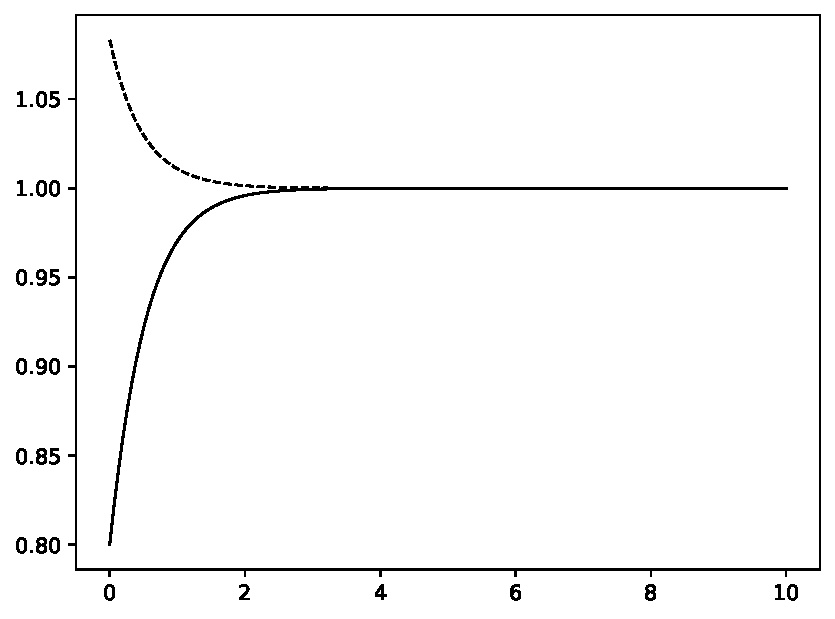
\includegraphics[scale=0.6]{figure_S_evolve.pdf}
	\caption{The evolution of $S_t$ in time $t$, given that $\lambda = 1$ and $\sigma = 1$.} \label{fig-S-evol}
\end{figure}



% Contest Deadline
Following \cite{ryvkin2022fight}, let's consider a dynamic contest with a given fixed deadline. 
Suppose the contest is terminated when time $t=T>0$. 
Since the variance $\bar{S}$ is fixed as assumed above, the state of the game is fully characterized by a tuple $(\tilde{y}_t, t)$. 
At any time $0\le t<T$, player $i$ optimizes her effort level $q_{i,\tau}$ in the remaining contest period $\tau\in[t, T)$ according to the following optimization problem, 
\begin{equation}\label{v-def}
	V^i(\tilde{y}_{t}, t ; q_{j,t},\Theta_i) = \max_{\{q_{i,\tau}\}^T_{\tau=t}} 
	\mathbb{E}\left( \theta\cdot1_{\tilde{y}_T>0} - \int^T_tC_i(q_{i,\tau})d\tau \bigg|I_t\right) 
\end{equation}
where $\Theta \equiv\{\theta, \lambda, \sigma, c_i, c_j\}$, subject to constraints (\ref{filtered-x}), (\ref{filtered-S}) and $q_{i,\tau}\ge0$ for all $\tau\in[t,T)$.
The optimization problem for player $j$ is just symmetric to that of player $i$ as $V^j(\tilde{y}_t, t) = V^i(-\tilde{y}_t, t)$. 
The corresponding Hamilton-Jacobi-Bellman (HJB) equation for player $i$ is 
\begin{equation*}
0 = \max_{q_{i,t}\ge0}\left[-\frac{c_iq_i^2}{2} + V^i_{y}\cdot\left(q_{i,t}-q_{j,t}\right)+V^i_t + \frac{V^i_{yy}}{2}\lambda \bar{S}^2\right]
\end{equation*}
Under the assumption of inner solution, we plug into the first order conditions $q_{i,t} = V^i_y/c_i$ and $q_{j,t} = -V^j_y/c_j$, we have the system of equations
\begin{equation*}
\begin{aligned}
\frac{1}{2c_i}(V^i_y)^2 + \frac{1}{c_j}V^i_yV^j_y + V^i_t + V^i_{yy}\frac{\lambda \bar{S}}{2} = 0\\
\frac{1}{2c_j}(V^j_y)^2 + \frac{1}{c_i}V^j_yV^i_y + V^j_t + V^j_{yy}\frac{\lambda \bar{S}}{2} = 0
\end{aligned}
\end{equation*}
subject to boundary conditions $V^i(-\infty, t) = 0$, $V^i(+\infty, t) = \theta$, $V^j(-\infty, t) = \theta$, $V^j(+\infty, t)=0$, $V^i(\tilde{y}_T, T) = \theta \cdot 1_{\tilde{y}_T > 0}$ and $V^j(\tilde{y}_T, T) = \theta \cdot 1_{\tilde{y}_T < 0}$. 


The Nash equilibrium is summarized in the following lemma: 

\begin{lemma}[\citealt{ryvkin2022fight}]
In the Markov perfect equilibrium, the players’ efforts in state $(\tilde{y}_t, t) \in\mathbb{R}\times[0, T)$ are given by
\begin{equation*}
m_{i}(\tilde{y}_t, t) = \frac{e^{-z_t^2/2}\lambda^{1/4}\sigma^{1/2}}{2\sqrt{2\pi(T-t)}} \cdot \left[\gamma(\rho_{i}) + \gamma(\rho_{j})\right]\left[1-\rho(z_t)^2\right]\left[1 + \rho(z_t)\right]
\end{equation*}
\begin{equation*}
m_{j}(\tilde{y}_t, t) = \frac{e^{-z_t^2/2}\lambda^{1/4}\sigma^{1/2}}{2\sqrt{2\pi(T-t)}} \cdot 
 \left[\gamma(\rho_{i}) + \gamma(\rho_{j})\right]\left[1-\rho(z_t)^2\right]\left[1 - \rho(z_t)\right]
\end{equation*}
where $z_t = \tilde{y}_t / \sqrt{\lambda^{1/2}\sigma(T-t)}$, $\rho(z_t) = \gamma^{-1}\left(\Phi(z_t)\left[\gamma(\rho_{i})+\gamma(\rho_{j})\right]-\gamma(\rho_{j})\right)$ and 
\begin{equation*}
\gamma(u) = \frac{u}{1-u^2} + \frac{1}{2}\ln\frac{1+u}{1-u},
\end{equation*}
\begin{equation*}
\rho_{i} = \frac{e^{w_{i}}+e^{-w_{j}}-2}{e^{w_{i}}-e^{-w_{j}}},
\quad
\rho_{j} = \frac{e^{w_{j}}+e^{-w_{i}}-2}{e^{w_{j}}-e^{-w_{i}}},
\quad
w_{i(j)} = \frac{\theta}{\lambda^{1/2}\sigma c_{i(j)}}.
\end{equation*}
\end{lemma}

We include a simplified version of the proof in the appendix.

...


\section{Model Estimation}

Unknown parameters to be estimated: 
\begin{itemize}
	\item $\sigma$ (Total innovation risk): 
	\item $\rho_i$ and $\rho_j$ (Capacities)
\end{itemize}

Likelihood: 
Data are submission times $\{t^i_k\}_{k=1}^{N_i}$ and $\{t^j_k\}_{k=1}^{N_i}$. 

We assume the submission times follow inhomogeneous Poisson process, controlled by the effort functions $\tau_i(t)$ and $\tau_j(t)$. 
Then, during any time interval of the contest $\mathcal{S}$, the Poisson arrival rate of submissions of the representative player $i$ is given by $\int_{s\in\mathcal{S}}\tau_i(s)ds$. 
The likelihood function of any realization of this point process $\{t^i_k\}_{k=1}^{N_i}$ is given by 
\begin{equation*}
p\left(\{t^i_k\}_{k=1}^{N_i} | \tau_i\right) = \exp\left\{-\int_{s\in\mathcal{D}}\tau_i(s)ds\right\}\prod_{k=1}^{N_i}\tau_i(t^i_k)
\end{equation*}






\section{Application}

...

\subsection{Synthetic Data}

Before applying our estimation procedure to real-world contest data, we evaluate its potential on synthetically generated data.



\subsection{Case Study}

...


\newpage
\section{Conclusion}

\newpage
\bibliography{_Literatures.bib}

\newpage
\appendix
\small

%{\footnotesize





\section{Solve $S_t$ in Equation (\ref{filtered-S})}\label{app-S-equ}

If $S$ is in steady state $dS/dt = 0$ $\Leftrightarrow$ $S = \bar{S} \equiv \sigma/\sqrt{\lambda}$. 
If $S$ is not in steady state, i.e. $S\not=\bar{S}$, we first isolate the two variables and get 
\begin{equation*}
	\frac{dS}{\sigma-\lambda S^2} = dt
\end{equation*}
Then, we take the integral on both sides
\begin{equation*}
    t = \int \frac{dS}{\sigma-\lambda S^2} = \frac{1}{\sigma\sqrt{\lambda}} \int \frac{dS\sqrt{\lambda}/\sigma}{1 - (S\sqrt{\lambda}/\sigma)^2} \equiv \frac{1}{\sigma\sqrt{\lambda}}\int \frac{du}{1-u^2} 
\end{equation*}
where $u = S\sqrt{\lambda}/\sigma = S/\bar{S}$. Hence, 
\begin{equation*}
    \sigma\sqrt{\lambda}\cdot t = \begin{cases}
        \tanh^{-1}(u)-K_1, & \text{if } |u|<1\\
        \coth^{-1}(u)-K_2, & \text{if } |u|>1
    \end{cases} = \begin{cases}
        \tanh^{-1}(S/\bar{S})-K_1, & \text{if } S<\bar{S}\\
        \coth^{-1}(S/\bar{S})-K_2, & \text{if } S>\bar{S} 
\end{cases}
\end{equation*}
Thus, we conclude the non-steady state case that 
\begin{equation*}
	S = \begin{cases}
		\bar{S}\cdot\tanh(\sigma\sqrt{\lambda}\cdot t + K_1), & \text{if } S<\bar{S}\\
		\bar{S}\cdot\coth(\sigma\sqrt{\lambda}\cdot t + K_2), & \text{if } S>\bar{S} 
	\end{cases}
\end{equation*}
Finally, we determine the constants $K_1$, $K_2$ by the initial condition $S_0$ and have 
\begin{align*}
	K_1 &= \tanh^{-1}(S_0/\bar{S})\\
	K_2 &= \coth^{-1}(S_0/\bar{S})
\end{align*}











\end{document}
